\documentclass{report}
\usepackage{settings}  % подклчючение настроек документа


% \usepackage{hyperref} % При желании
\usepackage{xurl} 
\def\UrlFont{\normalfont}

% Подавить бесполезные предупреждения
\hbadness=10000

\begin{document}

%%%% Вставка необходимого титульника %%%%
%\thispagestyle{titlepage} % Для размещения Иркутск в нижнем колонтитуле
%\newpage
    \begin{center}
    \linespread{1}
		Министерство науки и высшего образования  Российской Федерации\\
федеральное государственное бюджетное образовательное учреждение\\
высшего образования\\
«Иркутский государственный университет»\\
(ФГБОУ ВО «ИГУ»)\\
Факультет бизнес-коммуникаций и информатики 
    \end{center}
\vspace{1cm}    
\hspace{8cm} 
\begin{minipage}{0.5\textwidth}
\linespread{1}

  \begin{flushleft}
	\small{
    Кафедра естественнонаучных дисциплин \\%\vspace{-2cm}
Допускается к защите \\
и.о. зав. кафедрой, к.ф.-м.н., доцент \\
\rule{2,1cm}{0,1pt} А.Г. Балахчи\\		
            «\rule{0,9cm}{0,1pt}»\rule{2,7cm}{0,1pt} 202\,\rule{0,2cm}{0,1pt} г \\		}
		%\vspace{2еm}
		
		
		%\vspace{4.0em}
		\end{flushleft}
\end{minipage}


    \vspace{2cm} %вертикальное расстояние
    \begin{center}
   {\bf ВЫПУСКНАЯ КВАЛИФИКАЦИОННАЯ РАБОТА БАКАЛАВРА ИЛИ КУРСОВАЯ РАБОТА\\
    по направлению  \\
		09.03.03 Прикладная информатика\\
		%\vspace{1em}
		профиль\\
		«Название профиля»\\}
    \end{center}
		
		%\vspace{2.5em}%вертикальное расстояние
    \begin{center}
  		Название выпускной квалификационной работы или курсовой работы\\
    \end{center}
		
		\vspace{2.5em}
		
   \hspace{-5em} 


\noindent
\begin{minipage}[t]{0.5\textwidth}
  \begin{flushleft}
  \linespread{1}
	\small{
    Консультант: должность, ученое звание \\
  Место работы\\
        \rule{1,8cm}{0,1pt} ФИО (в именительном падеже)\\
	\vspace{2em}
		
	Нормоконтролёр: должность, уч. зв,\\
            \rule{1,8cm}{0,1pt} ФИО (в им. падеже)\\
}
		%\vspace{2em}
		
		
		%\vspace{4.0em}
		\end{flushleft}
\end{minipage}%\hspace{1em} 
\begin{minipage}[t]{0.5\textwidth}
  \begin{flushleft}
  \linespread{1}
	\small{
    Студент ** курса
	** формы обучения \\
  группа **\\
        \rule{1,8cm}{0,1pt} ФИО (в им. падеже)\\
	\vspace{2em}
		
	Руководитель: уч. степень, уч. звание\\
            \rule{1,8cm}{0,1pt} ФИО (в им. падеже)\\
\vspace{2em}
 Работа защищена:\\
        «\rule{0,9cm}{0,1pt}»\rule{2,7cm}{0,1pt} 202\,\rule{0,2cm}{0,1pt} г \\
с оценкой \rule{1,8cm}{0,1pt}\\
Протокол № \rule{0,9cm}{0,1pt}}
		%\vspace{2em}
		
		
		%\vspace{4.0em}
		\end{flushleft}
\end{minipage}
\vfill

% Изменить год в надписи <<Иркутск 202*>> нужно в файле settings.sty на 221 строке

\newpage  % Титульный лист дипломной работы 
%\thispagestyle{titlepage}
%\newpage

    \begin{center}
    \linespread{1}
		Министерство науки и высшего образования  Российской Федерации\\
федеральное государственное бюджетное образовательное учреждение\\
высшего образования\\
«Иркутский государственный университет»\\
(ФГБОУ ВО «ИГУ»)\\
Факультет бизнес-коммуникаций и информатики 
    \end{center}
\vspace{1cm}    
\hspace{8cm} 
\begin{minipage}{0.5\textwidth}
\linespread{1}
%подписи для ВКР в курсовой можно удалить или заменить на настройку вертикального расстояния
  \begin{flushleft}
	\small{
    Кафедра естественнонаучных дисциплин \\%\vspace{-2cm}
Допускается к защите \\
и.о. зав. кафедрой, к.ф.-м.н., доцент \\
\rule{2,1cm}{0,1pt} А.Г. Балахчи\\		
            «\rule{0,9cm}{0,1pt}»\rule{2,7cm}{0,1pt} 202\,\rule{0,2cm}{0,1pt} г \\		}
		%\vspace{2еm}
		
		
		%\vspace{4.0em}
		\end{flushleft}
\end{minipage}


    \vspace{2cm} %вертикальное расстояние
    \begin{center}
   {\bf ВЫПУСКНАЯ КВАЛИФИКАЦИОННАЯ РАБОТА БАКАЛАВРА ИЛИ КУРСОВАЯ РАБОТА\\
    по направлению  \\
		09.03.03 Прикладная информатика\\
		%\vspace{1em}
		профиль\\
		«Название профиля»\\}
    \end{center}
		
		%\vspace{2.5em}%вертикальное расстояние
    \begin{center}
  		Название выпускной квалификационной работы или курсовой работы\\
    \end{center}
		
		\vspace{2.5em}
		
   \hspace{-5em} 


\noindent
\begin{minipage}[t]{0.5\textwidth}
  \begin{flushleft}
  \linespread{1}

		%\vspace{2em}
		
		
		%\vspace{4.0em}
		\end{flushleft}
\end{minipage}%\hspace{1em} 
\begin{minipage}[t]{0.5\textwidth}
  \begin{flushleft}
  \linespread{1}
	\small{
    Студент ** курса
	** формы обучения \\
  группа **\\
        \rule{1,8cm}{0,1pt} ФИО (в им. падеже)\\
	\vspace{2em}
		
	Руководитель: уч. степень, уч. звание\\
            \rule{1,8cm}{0,1pt} ФИО (в им. падеже)\\
\vspace{2em}
 Работа защищена:\\
        «\rule{0,9cm}{0,1pt}»\rule{2,7cm}{0,1pt} 202\,\rule{0,2cm}{0,1pt} г \\
с оценкой \rule{1,8cm}{0,1pt}\\
Протокол № \rule{0,9cm}{0,1pt}}
		%\vspace{2em}
		
		
		%\vspace{4.0em}
		\end{flushleft}
\end{minipage}

    \vfill
% Изменить год в надписи <<Иркутск 202*>> нужно в файле settings.sty на 221 строке
    
\newpage  % Титульный лист курсовой работы

\includepdf[pages={1}]{TitlePages/praktika.pdf} % Ваш титульний лист в .pdf 

%(если ваш титульный лист в формате .docx - воспользуйтесь сервисом по конвертации из docx (Word) в pdf)


\setcounter{page}{2} % начинаем нумерацию страниц
\tableofcontents  % это содержание, которое генерируется автоматически

\setcounter{chapter}{0} % установка счетчика глав
\setcounter{section}{0} % установка счетчика разделов
\setcounter{subsection}{0} % установка счетчика подразделов
\setcounter{equation}{0} % установка счетчика формул


\chapter*{ВВЕДЕНИЕ} % звездочка нужна, чтобы не было нумерации у этой главы
\addcontentsline{toc}{chapter}{ВВЕДЕНИЕ} % чтобы глава отображалась в содержании

В ИСЗФ СО РАН имеется уникальная научная установка --- Иркутский Радар Некогерентного Рассеяния (ИРНР). Всего в мире существует несколько подобных радаров, а ИРНР --- единственный в России. Данный инструмент является большой радиолокационной станцией, используемой для изучения процессов, происходящих в ионосфере Земли, а также для экспериментов по наблюдению за космическими объектами. Ниже представлены ключевые характеристики ИРНР из источника \cite{irnr1}.

\begin{enummarker}
    \item Диапазон рабочих частот: 154--162 МГц.
    \item Пиковая мощность, достигаемая на двух передатчиках: 2.8 МВт.
    \item Длительность зондирующего импульса: от 70 до 900 мкс.
    \item Частота следования импульсов: 24.4 Гц.
    \item Коэффициент усиления антенны: около 35 дБ.
\end{enummarker}

Радиолокационные станции являются сложными системами с большим количеством компонентов и разнятся по своей структуре. В общем случае, принцип действия радиолокационной станции заключается в излучении мощного зондирующего импульса и получении маломощного эхо, отразившегося от среды или объекта. В излучении участвует задающая часть, передатчики и антенна, совместно образующие передающий тракт --- набор компонентов, через которые проходит путь следования сигнала при излучении. Для приёма задействуется приёмный тракт, который состоит из антенны, усилителей, фильтров и регистрирующего комплекса.

Влияние приёмного и передающего тракта на проходящие через них сигналы прямым образом сказывается на способности радиолокационной станции получать достоверные данные в процессе наблюдений. В силу своей неидеальной природы, оборудование может искажать сигналы, ослаблять их и вносить задержки --- что очень критично в задачах с высокими требованиями к точности, например при определении расстояния до объекта на орбите на основе задержки радарного эхо.

В связи с этим возникает потребность в регулярной диагностике оборудования для оценки его характеристик (задержка, амплитудно-частотная характеристика, фазо-частотная характеристика и их стабильность) чтобы учесть их в дальнейшем на этапе обработки полученных данных. Кроме того, высокочувствительное оборудование приёмного тракта может быть легко повреждено в силу своей близости к мощному излучению передатчиков, в связи с чем также возникает потребность в возможности быстрого обнаружения отказов приёмного тракта, что позволило бы обеспечить своевременное проведение ремонтных работ и помогло бы снизить общее время простоя.

Подобные потребности присущи не только ИРНР, но радиолокационным станциям в целом. Как правило, они решаются при помощи встроенных и тесно интегрированных средств диагностики, приспособленных под особенности строения конкретной станции. На текущий момент в составе ИРНР нет отдельной системы для диагностики приёмного тракта, и задача измерения его характеристик решаются при помощи методов пассивной калибровки по излучению звёздных радиоисточников, что обладает ограниченной оперативностью, а обнаружение отказов происходит путём визуального осмотра получаемых в процессе наблюдений данных, что тоже обладает ограниченной оперативностью.

Для более тщательного решения данных задач в рамках ИРНР, предлагается разработка узкоспециализированного программно-аппаратного комплекса для диагностики и исследования характеристик его приёмного тракта. В состав комплекса входит программируемый генератор тестовых сигналов, построенный на основе цифрового синтезатора сигналов AD9910 и микроконтроллера STM32 со встроенным ПО на языке программирования Си, а также пакет программных инструментов для управления и аналитики на языке программирования Python.

Принцип действия системы заключается в использовании программируемого генератора сигналов для подачи тестовых сигналов известной формы на вход приёмного тракта ИРНР и использовании штатного регистрирующего комплекса радара для получения записей сигналов. Затем, на основе анализа различий между полученным в действительности сигналом и прогнозировавшимся на основе модели сигналом выполняется оценка характеристик приёмного тракта.

Внедрение подобного решения на постоянной основе позволило бы регулярно выполнять активную калибровку приёмного тракта ИРНР и с высокой оперативностью проводить диагностику в случае возникновения подозрений на отказ оборудования. В дальнейшем, информация о характеристиках приёмного тракта может использоваться для повышения точности измерений в научных задачах.

{\bf Объект исследования:} комплексная передаточная функция радиофизической системы.

{\bf Предмет исследования:} амплитудно-частотная характеристика (АЧХ) и фазо-частотная характеристика (ФЧХ) антенно-фидерного тракта Иркутского радара некогерентного рассеяния (ИРНР).

{\bf Цель исследования:} создание программно-аппаратного комплекса, позволяющего проводить оперативные измерения АЧХ и ФЧХ антенно-фидерного тракта, что существенно улучшит диагностические возможности ИРНР. Программно-аппаратный комплекс должен предусматривать возможность использования в составе ИРНР на постоянной основе.

{\bf Задачи:}
\begin{enumarabic}
\item расширение возможностей разработанного ранее программируемого генератора тестовых сигналов;
\item разработка гибкого форматов файлов конфигураций для описания диагностических сценариев;
\item разработка программных инструментов для проведения измерений и получения результатов в полуавтоматическом режиме.
\end{enumarabic}


{\bf Теоретическая новизна исследования} заключается в разработке приспособленных под особенности ИРНР подходов к проведению диагностических измерений, в разработке методов управления для применения цифрового синтезатора сигналов AD9910 в роли многоцелевого генератора тестовых сигналов, разработке форматов данных для описания сложных диагностических сценариев с использованием программируемого генератора сигналов.

{\bf Практическая значимость исследования} заключается в развитии диагностических возможностей ИРНР.

% 
\setcounter{section}{0} % обнуление счетчика разделов перед новой главой
\setcounter{subsection}{0} % обнуление счетчика подразделов перед новой главой
\setcounter{equation}{0} % обнуление счетчика формул перед новой главой

\chapter{КОНЦЕПЦИЯ СИСТЕМЫ ДИАГНОСТИКИ ПРИЕМНОГО ТРАКТА}

\section{Краткий обзор предметной области}

Архитектура каждой отдельно взятой радиолокационной станции зависит от специфики выполняемых задач, но в общем случае радиолокационные станции являются технологически сложными системами, сочетающими в себе высокие требования к мощности создаваемого излучения и высокие требования относительно чувствительности к получаемому излучению. Компоненты в составе РЛС подвержены воздействиям, которые редко встречаются где-либо ещё.

Время между излучением зондирующего импульса и получением отражённого сигнала часто составляет малые доли секунды, что также приводит к большим требованиям касательно синхронизации между передающим и приёмным оборудованием станции.

Естественное старение и работа в сложных условиях приводят к износу оборудования, что может выражаться как в постепенной деградации отдельных компонентов, так и в неожиданных отказах. Также играет роль человеческий фактор --- возможно допущение ошибок, особенно во время обслуживания оборудования, что может заключаться, например, в неправильном подключении кабелей. Всё это может ухудшить качество получаемых данных или вообще воспрепятствовать проведению наблюдений.

В связи с этим радиолокационные станции обычно имеют в своём составе диагностические средства, которые призваны помочь в оценке состояния оборудования. Их набор может включать всё от измерительных устройств для проверки состояния отдельных элементов системы до генераторов тестовых сигналов, которые тестируют группы компонентов в сквозном режиме.

Приёмный тракт станции является одной из подсистем, которые целесообразно тестировать в сквозном режиме. Роль приёмного тракта заключается в усилении слабых сигналов полученных антенной и их преобразовании в вид, который пригоден для дальнейшей обработки в рамках регистрирующего комплекса. Приёмный тракт, в частности его отдельные каналы, обладают последовательным строением: подключенные друг за другом ключи, фильтры, усилители, и связующие их кабели. Характеристики приёмного тракта являются произведением характеристик всех его частей, и отказ одного элемента приведёт к неработоспособности всего тракта.

Диагностические средства можно разделить на три категории по величине того, насколько их использование препятствуют проведению обычных наблюдений:

\begin{enummarker}
    \item не препятствуют вовсе;
    \item требуют временного приостановления наблюдений;
    \item требуют внесения изменений в аппаратную конфигурацию станции.
\end{enummarker}

Некоторые диагностические средства, например датчики тока или мощности, могут использоваться непосредственно в процессе наблюдений, поскольку имеют исключительно пассивный характер действия. Другие могут потребовать отключения передатчиков станции. Наконец, наиболее инвазивными являются те, которые требуют переподключения кабелей или иного вмешательства в работу оборудования. Для диагностики приёмного тракта можно представить сценарии со всеми тремя категориями тестов, что будет подробнее раскрыто далее.

В целом, проблема диагностики радиолокационных станций и приёмного тракта в частности не нова. В литературе можно найти описания диагностических систем существовавших в прошлом радиолокационных станций \cite{abm}. Известно, что РЛС Днепр, которая лежит в основе ИРНР, предусматривала средства для тестирования приёмного тракта, однако они не сохранились после множества модернизаций и в любом случае были бы устаревшими по современным меркам.

С точки зрения пропускания сигналов, основными характеристиками  приёмного тракта (и его составляющий частей) можно считать амплитудно-частотную характеристику и фазо-частотную характеристику.

Амплитудно-частотная характеристика (АЧХ) определяется ослаблением или усилением, которое представлено выраженным от частоты коэффициентом. Усилением обладают, как правило, только усилители. Фильтры ослабляют сигналы, причём таким образом, чтобы исключить нежелательные частоты и оставить только желаемые. Усиление приёмного тракта напрямую влияет на то, насколько слабые сигналы может обнаружить станция.

Фазо-частотная характеристика (ФЧХ) определяется смещением фазы между сигналом на входе и сигналом на выходе, в зависимости от частоты, что, в свою очередь, напрямую определяется задержкой, которую вносит устройство. Причём, одинаковая задержка вызовет более сильное смещение фазы для колебаний, которые выше по частоте. В связи с тем, что скорость распространения сигналов конечна, кабели любой длины будут обладать некоторой ФЧХ.

% TODO: доп. про почему важно усиление

Данные характеристики можно присвоить любым системам, которые работают с сигналами, в частности цифровым фильтрам. В цифровом представлении, несложно получить идеальное усиление или ослабление сигналов: достаточно умножить на выбранный коэффициент значения сигнала от времени, и результатом будет усиление или ослабление всех частот в сигнале. Похожим образом можно с абсолютной точностью измерить характеристики цифровых систем преобразования сигналов.

Реальный приёмный тракт, однако, состоит из реальных устройств, которые работают с токами высокой частоты (радиочастотных устройств). На высоких частотах паразитные ёмкости и паразитные индуктивности начинают играть большую роль и затрудняют измерения, в связи с чем измерение АЧХ и ФЧХ реальных устройств на высоких частотах считается сложной задачей, к которой нужно подходить с большой осторожностью.

% токи высокой частоты: нужен источник
% радиочастотные устройства: нужен источник
% считается сложной задачей: нужен источник

\section{Специфика ИРНР}

В контексте ИРНР, амплитудно-частотная характеристика и фазо-частотная характеристика приёмного тракта оказывают влияние на точность оценки пространственного положения источников сигнала в поле зрения антенны.

Антенна ИРНР является антенной с частотным сканированием, то есть это антенна, которая может электронно изменять направление луча, несмотря на своё фиксированное положение в пространстве. Во время излучения, отклонение луча вдоль большой оси антенны происходит при помощи изменения частоты сигнала. Во время приёма, антенна обладает зависящей от частоты чувствительностью для каждого возможного угла в поле зрения вдоль большой оси.

Можно представить ситуацию, когда в антенну ИРНР под некоторым углом вдоль большой оси приходит сигнал с равным содержанием всех частот; исходя из того, на какой частоте антенна воспримет больше всего мощности, можно установить угол. Однако вследствие неравномерного усиления приёмного тракта, некоторая ложная частота может быть воспринята как частота с максимальной мощностью, что помешает точной оценке угла. В связи с этим желательно знать и учитывать амплитудно-частотную характеристику приёмного тракта.

Другим методом происходит определение угла вдоль малой оси антенны. Внутренне антенна при помощи перегородки разделена на два полурупора, которые образуют два канала приёма. Когда сигнал достигает антенны под некоторым углом вдоль малой оси, он достигнет дальний полурупор с некоторой задержкой относительно ближнего полурупора, что приведёт к возникновению разности фаз между полурупорами и соответствующими им каналами, причём разность пропорциональна углу. Таким образом, определив разность фаз можно определить угол. Однако два канала приёмного тракта вносят собственную задержку в сигнал, и если задержка между ними различается, то наблюдаемая на выходе разность фаз изменится от исходной, что также помешает точной оценке угла. На высоких частотах, небольшие различия в длине кабелей и производственный разброс характеристик между номинально одинаковыми компонентами могут создавать различия между внешне одинаковыми по строению каналами приёмного тракта. В связи с этим желательно знать и учитывать фазо-частотную характеристику приёмного тракта.

Представленные ранее проблемы решаются методами пассивной калибровки по излучению космических радиоисточников, которые позволяют установить соответствие между достоверно известным положением объектов на небе и тем, что воспринимает оборудование станции. Это не отменяет потребности в системе диагностики для приёмного тракта; наличие средства для активной калибровки стало бы хорошим дополнением к методам пассивной калибровки.

Из этого исходят два основных сценария использования диагностической системы в рамках ИРНР:

\begin{enummarker}
    \item оценка АЧХ;
    \item оценка ФЧХ (в частности разности фаз между каналами).
\end{enummarker}

Широко используемым инструментом для оценки АЧХ и ФЧХ являются векторные анализаторы цепей (VNA), которые представляют собой готовое решение специально предназначенное для выполнения данной задачи. Чаще всего они существуют в форме автономного устройства, но встречаются также варианты, подключаемые к компьютеру.

В векторных анализаторах цепей вводится понятие исследуемого устройства: набора из одного или нескольких компонентов, характеристики которых требуется оценить. Также вводится понятие портов, которое обозначает входы/выходы векторного анализатора. Большинство векторных анализаторов являются двухпортовыми устройствами и предполагают подключение входа исследуемого устройства к первому порту, а выхода ко второму порту. По своей внутренней структуре векторные анализаторы содержат собственный генератор тестовых сигналов с настраиваемой мощностью, и несколько работающих синхронно чувствительных приёмников, обладающих возможностью одинаково воспринимать поступающие сигналы, но подключенных по-разному.

Принцип действия VNA заключается в подаче сигнала на вход исследуемого устройства и измерении, одновременно, комплексных амплитуд (амплитуды и фазы) падающего сигнала, отраженного сигнала, и прошедшего через исследуемое устройство сигнала, которые попадают в соответствующие приёмники напрямую или при помощи направленных ответвителей \cite{vna1}. На основе отношения комплексных амплитуд вычисляются так называемые S-параметры, которые описывают АЧХ и ФЧХ исследуемого устройства. Данное измерение происходит на множестве частот в цикличном режиме, и программное обеспечение VNA предусматривает возможность усреднения по пройденным несколько раз точкам, чтобы исключить влияние шума.

Многие векторные анализаторы цепей используют непрерывный сигнал, но существуют также импульсные VNA, которые могут подавать короткие импульсы по внешнему синхронизационному сигналу. Импульсный режим встречается только на более дорогих устройствах, но необходим в сценарии с использованием на ИРНР в связи с одной уникальной особенностью окружающей среды --- поблизости расположена другая радиолокационная станция, работа передатчиков которой создаёт мощные помехи для работы любого измерительного оборудования, не интегрированного со специальной системой синхронизации между двумя станциями.

Вне зависимости от стоимости, набор функций в готовых VNA фиксирован и не предполагает возможности расширения. Кроме того, сопутствующее ПО не имеет открытого исходного кода, что ограничивает возможности по организации взаимодействия с другим ПО в целях автоматизации.

В контексте диагностического средства для приёмного тракта ИРНР, векторный анализатор цепей нельзя использовать для сквозного тестирования вместе со штатным регистрирующим комплексом станции, поскольку VNA требует, чтобы выход исследуемого устройства был подключен только к его собственному приёмнику. Это исключает возможность измерений без перекоммутации кабелей, что крайне нежелательно --- любое изменение конфигурации оборудования сильно усложняет процедуру проведения диагностики и создаёт риск человеческой ошибки, выраженной, например, в перепутанных местами кабелях в результате невнимательности, с непреднамеренной потерей ценных научных данных в результате запуска станции в неправильно сконфигурированном состоянии после проведения диагностики.

В связи с высокой стоимостью подобных устройств, а также обозначенными выше недостатками, вариант использования коммерческого векторного анализатора в роли диагностического средства для приёмного тракта ИРНР считается несостоятельным.

Вместо этого выбран вариант разработки тесно интегрированного программно-аппаратного комплекса, обладающего упрощённым набором функций по сравнению с векторными анализаторами (измерение характеристик только прошедшего сигнала), но предоставляющего схожие возможности по измерению характеристик приёмного тракта. Главным преимуществом тесной интеграции с имеющимися системами радара является использование штатного регистрирующего комплекса и исключение необходимости в перекоммутации, что позволяет проводить диагностику без внесения изменений в конфигурацию оборудования станции.

В состав программно-аппаратного комплекса входит программируемый генератор тестовых сигналов, штатный регистрирующий комплекс радара, и программный пакет для управления и аналитики, который предоставляет возможности по автоматизации выполнения типовых диагностических сценариев, а также программные инструменты для анализа получаемых в процессе диагностики данных.

С точки зрения задачи оценки АЧХ и ФЧХ приёмного тракта, принцип действия данного решения заключается в использовании программируемого генератора сигналов для подачи сигналов известной формы на вход приёмного тракта и использовании регистрирующего комплекса для записи сигналов после прохождения через весь приёмный тракт. Исходя из отношения параметров полученного в действительности сигнала к параметрам модельного либо иного опорного сигнала, возможна оценка АЧХ и ФЧХ.

К генератору сигнала предъявляются определённые требования. Во-первых, он должен обладать возможностью создания сигналов в рабочем диапазоне частот станции, поскольку оценка АЧХ и ФЧХ требуется в этом диапазоне. Во-вторых, от него требуется возможность создавать короткие импульсы по внешнему событию от системы синхронизации станции. Длительность импульсов должна быть схожа с длительностью стандартных зондирующих импульсов --- необходимо, чтобы импульс излучился одновременно с началом записи и вместился по длительности в окно записи регистрирующего комплекса. В третьих, от генератора сигналов требуются возможность создания импульсов с линейной частотной модуляцией. В целом ожидается наличие возможностей по имитации штатных зондирующих импульсов станции.

% для подключения генератора сигналов к приёмному тракту предполагается задействовать служебные входы в антенной системе, чтобы не изменять коммутацию самого приёмного тракта?

На рынке доступно множество генераторов сигналов, которые предназначены для выполнения различных задач, от простых до очень сложных \cite{siggen1} \cite{siggen2}. Простейшие генераторы сигналов предназначены только для создания непрерывных сигналов на выбранной частоте и с выбранной амплитудой. Ключевыми характеристиками таких генераторов является диапазон поддерживаемых частот и уровней амплитуды. Более сложные генераторы обладают возможностями по модуляции сигналов, то есть изменению их параметров по внешнему событию либо по предопределённому набору правил. Здесь важным критерием становится интерфейс, через который осуществляется управление модуляцией, и его ограничения. Наконец, существуют векторные генераторы сигналов, которые позволяют создавать несколько сигналов (точнее, колебаний) и обычно используются при разработке телекоммуникационного оборудования.

Использование векторных генераторов сигналов не оправдывается поставленными ранее требованиями, но в то же время данные требования исключают все недорогие варианты. В целом, вариант использования рыночного генератора сигналов в рамках системы диагностики сталкивается со схожими проблемами, что и вариант использования рыночного VNA. Большинство доступных на рынке генераторов сигналов выполнены в виде автономных устройств, которые предусмотрены для использования в роли лабораторного инструмента, а не для интеграции в состав другой системы.

В связи с этим ранее был разработан собственный программируемый генератор сигналов. Он представляет собой управляемое через USB или Ethernet устройство на основе микроконтроллера STM32 и цифрового синтезатора частот AD9910. Встроенное ПО генератора сигналов написано на языке программирования Си и реализует интерфейс конфигурации при помощи текстовых команд и различные режимы работы.

Штатный регистрирующий комплекс является многоканальной системой оцифровки и записи сигналов, находящейся в активной эксплуатации и играющей критическую роль в выполнении  задач станции. Внесение изменений в ПО регистрирующего комплекса связано с риском добавления скрытых дефектов, которые могут нарушить выполнение научных задач. Решено никак не изменять его текущее ПО для адаптации под нужды системы диагностики и использовать только те интерфейсы взаимодействия, которые доступны сейчас.

Пакет управления и аналитики включает в себе программные инструменты, которые реализуют поддержку основных сценариев использования программно-аппаратного комплекса.

Процесс работы с системой с точки зрения оператора станции можно разделить на два этапа: получение данных и анализ данных. На этапе получения данных происходит подача тестовых сигналов в приёмный тракт и запись прошедших через приёмный тракт сигналов. На этапе анализа данных происходит обработка записей и построение графиков, либо сохранение полученных после обработки результатов в формат, пригодный для использования с другими инструментами.

В теории, программно-аппаратный комплекс может поддерживать некоторые сценарии, когда диагностика выполняется совместно со штатными наблюдениями, но это выходит за рамки данной работы. На текущем этапе проведение диагностики приёмного тракта предполагается выполнять только по запросу оператора после выполнения им ряда шагов по приостановке процесса выполнения обычных наблюдений. Иными словами, полная автоматизация процедуры диагностики приёмного тракта не предполагается.

При условии готовности оборудования --- то есть, когда передатчики станции выключены и регистрирующий комплекс не выполняет никаких других задач --- система диагностики может использоваться для проведения измерений с приёмным трактом. На рисунке \ref{fig:workflow1} изображено то, как задумывается взаимодействие оператора с компонентами программно-аппаратного комплекса, когда требуется получить график АЧХ приёмного тракта.

\myfigure{0.7}{workflow1.png}{Диаграмма деятельности для получения графика АЧХ}{workflow1}

На основе изучения полученного графика оператор может сделать вывод о текущем состоянии приёмного тракта и принять решение о необходимости выполнения дальнейших действий по диагностике в случае обнаружения проблем.

% Требования:
% - В рабочем диапазоне частот станции
% - Длительностью 900 мкс

% План по содержанию:
% ЧАСТЬ 1. ОБЗОР ПРЕДМЕТНОЙ ОБЛАСТИ
% - Задачи диагностики радаров
%     - История
%         - Конечно
%     - Возможности
%         - Группы тестов
% - Характеристики РЧ устройств
% - Специфика измерений на ИРНР
%     - Характеристики ИРНР
%     - Затухание
%     - Разность фаз между каналами
% - Векторные анализаторы спектра
%     - Трудности
% - Векторные генераторы сигналов
%     - Дорогие
%     - В итоге сделали свой

% ЧАСТЬ 2. АЛГОРИТМЫ

% - Регистрирующий комплекс даёт IQ
% - Мы делаем графики из IQ

% Что ещё следует покрыть:
% сценарии использования программно-аппаратного комплекса
% выявлен предположительный сценарий для диагностики
%   - скорее всего, будет один или два основных сценариев
%       - пробежка по рабочему диапазону ЛЧМ сигналами той или иной ширины
%   - с точки зрения инженера
%   - с точки зрения оператора станции при поддержке инженера
%       - нужен алгоритм действий
%       - и нужно проще
%   - получение записей+метаданных
%   - построение графика
%   - визуальное сравнение
%   - принятие решения в случае выявления проблем
% путь сигнала
% цифровая обработка

% алгоритмы
%    амплитудно-частотной характеристики
%    разности фаз

\section*{Выводы по главе}
\addcontentsline{toc}{section}{Выводы по главе}

В данной главе была кратко рассмотрена проблематика диагностики радиолокационных станций в целом и особенности диагностики ИРНР в частности. Углублённо рассмотрены потребности по диагностике приёмного тракта ИРНР. Представлена концепция программно-аппаратного комплекса для исследования характеристик приёмного тракта ИРНР, приведено развернутое обсуждение альтернативных подходов к решению проблем диагностики, и рассмотрены возможные сценарии использования.

\chapter{РАЗРАБОТКА СИСТЕМЫ ДИАГНОСТИКИ ПРИЕМНОГО ТРАКТА}
% снова обнуляем счетчики section, subsection и equation в новой главе
\setcounter{section}{0}
\setcounter{subsection}{0}
\setcounter{equation}{0}
\section{Расширение возможностей генератора сигналов}

% Что нужно покрыть:
% - Расширение возможностей генератора сигналов
%   - Что побудило?
%       - Неполнота
%       - Не раскрывает истинных возможностей оборудования
%       - Требует внесения изменений в программный код для новых видов сигналов
%       - Следовательно не обладает достаточной гибкостью для поддержки
%       непредусмотренных заранее тестовых сценариев
%   - Пересмотр подхода к управлению синтезатором
%       - Что побудило?
%       - Предпринята попытка рефакторинга
%       - Что поняли?
%   - Генератор логической последовательности
%       - Алгоритм дробления больших интервалов
%   - Крайне общее решение
%       - Позволяет реализовать поверх себя любые односторонние цифровые интерфейсы
%       - При этом подходит для задач, где требуется точная привязка ко времени
%       - Хорошо подходит для управления специализированными микросхемами, такими как AD
%   - Удобный программный интерфейс (картинка)
%   - Парсер JSON с низким использоваием оперативной памяти
%       - jsmn является лексером, который переводит документ в промежуточное представл.
%       - размечает на токены различных типов
%       - использование промежуточного представления требует оперативной памяти
%   - Соображения по взаимодействию
% - Интеграция с регистрирующим комплексом
%   - Соображения о режимах сканирования
%   - Проблема синхронного старта
%   - Ранее проблемой не являлось, связано с цикличным сканированием по сетке час.
%   - Режим следования за DDC
%       - Демон событий DDC
% - Формат файлов
%   - Абстракция
%   - Хочется следующее:
%   - Человеко-читаемый
%   - Гибкий и раскрывающий главные возможности оборудования
% - Инструмент контроля и управления
%   - Архитектура
%       - Файлы конфигураций диагностических сценариев
%       - Интерпретаторы сценариев
% - Адаптация аналитических иструментов

Разработанный ранее генератор сигналов предусматривает управление при помощи текстовых команд, которые передаются на вход несложному интерпретатору, вызывающему различные обработчики на основе названия команды. Набор команд генератора сигналов включает несколько служебных команд и ряд команд для осуществления операций по управлению очередью воспроизведения сигналов, которая называется секвенсором.

Поддерживаются несколько предопределённых видов сигналов: непрерывный сигнал, простой импульс, импульс с линейной частотной модуляцией, импульс с некоторым кодом фазовой манипуляции, и импульс с некоторым кодом частотной манипуляции.

Команды по добавлению сигналов в очередь воспроизведения принимают на вход набор перечисленных через пробел параметров и заполняют на их основе внутреннюю структуру данных, которая используется для представления сигналов в памяти микроконтроллера.

Преимуществом подобного подхода к конфигурации генератора сигналов является невысокая сложность, однако подобный интерфейс с несколькими жестко заданными видами сигналов не раскрывает истинных возможностей оборудования, требует внесения изменений в программный код для добавления поддержки новых видов сигналов, и в целом не обладает достаточной гибкостью для поддержки непредусмотренных заранее тестовых сценариев.

В связи с этим решено разработать улучшенный интерфейс управления генератором сигналов, который даёт более полный доступ к внутренней структуре данных для сигналов. Перед этим также решено пересмотреть нижележащие подходы к управлению цифровым синтезатором сигналов так, чтобы получить максимальную возможную гибкость в управлении и попробовать устранить некоторые недостатки. Здесь речь заходит уже об интерфейсе между микроконтроллером и синтезатором.

Генератор сигналов с самой первой итерации преследуют сложности, связанные с манипуляциями профильными входами синтезатора AD9910. Напомним, у синтезатора есть три логических входа для выбора профиля, которые позволяют выбрать один из восьми профилей со значениями амплитуды, частоты и фазы, либо с начальными и конечными адресами воспроизведения из оперативной памяти синтезатора, когда оперативная память задействована.

Манипуляция профилями во время импульса и воспроизведение из оперативной памяти являются двумя основными способами получения импульсов с модуляцией. Воспроизведение из оперативной памяти позволяет создавать некоторые виды импульсов в автономном режиме работы синтезатора, когда не требуется внешнего воздействия на входы на протяжении излучения, что позволяет исключить влияние временных нестабильностей в манипуляции входами со стороны микроконтроллера и получить сигналы детерминированной формы. Однако не все виды импульсов можно создать только с использованием оперативной памяти в связи с ограничениями, которые вытекают из ширины машинных слов памяти: 32-битная оперативная память может выступать источником 16+14-битных значений фазы и амплитуды, либо 32-битных значений частоты, но не одновременно. Импульсы, которые требуют частотной и фазовой манипуляции, в частности штатный зондирующий импульс радара, невозможно представить только с использованием оперативной памяти.

Для имитации штатного зондирующего импульса требуется использование манипуляции профилями. В рамках данного подхода наблюдаются две трудности: переключение состояния более одного профильного входа за раз с высокой вероятностью приводит к выбору неправильного профиля (это очень критично), а при переключении только одного профильного входа, хотя выбор профиля происходит корректно, моменты применения новых параметров сигнала перемещаются во времени, что характеризуется нестабильностью формы сигнала вблизи моментов переключений. Данные трудности, скорее всего, являются последствиями общей проблемы, которая кроется в несоблюдении требований ко времени установки и удержания уровней на профильных входах относительно тактовой частоты синтезатора, даже несмотря на внедрение общего источника тактирования.

На данный момент проблема считается фундаментальной к использованному микроконтроллеру и не подлежит исправлению. В качестве меры борьбы с проблемой предлагается рассматривать индекс активного профиля не как свободно выбираемый, а как увеличиваемый/уменьшаемый, с использованием кода Грея при переборе состояний профилей, чтобы исключить возможность переключения более одного входа за раз.

Данный вывод был получен после исключения другой потенциальной причины: было выдвинуто предположение, что по крайней мере часть проблемы может быть связана с неопределенностью задержек при выполнении блоком DMA транзакций по шине данных микроконтроллера, что может привести к нестабильности момента изменения профилей во времени и было схоже с наблюдаемым поведением. Задержки шины данных могут меняться от загруженности \cite{stm32dmalatency} и их трудно предсказать в сложной системе на чипе, какой является STM32. Выставление состояний профилей в тот момент происходило посредством записей заранее подготовленных значений в регистры GPIO посредством механизма DMA. Источником DMA запросов служил таймер модуляции, который запускался на период излучения и создавал события через равные промежутки времени.

Был разработан новый способ выставления профилей который полагается на каналы сравнения таймеров и позволяет буферизовать одно будущее состояние и точно привязать момент его принятия ко времени, тем самым минуя неопределенность шины данных. Принцип действия данного способа заключается в следующем: выбранный таймер, каналы сравнения которого могут быть использованы как аппаратные выходы, настраивается в режиме отсчитывающего вниз счётчика. Во все каналы сравнения загружается значение ноль, а режим канала выбирается так, чтобы при совпадении, выходу был присвоен либо низкий, либо высокий уровень. В регистр периода таймера загружается значение, соответствующее длительности промежутка времени, на протяжении которого каналы должны удерживать назначенные им состояния, а в регистр пока что незапущенного счётчика загружается единица. При запуске, каналы таймера спустя один такт примут заданные заранее значения, а таймер сгенерирует событие обновления и начнёт отсчитывать от заданного времени удержания состояний до нуля. В то же время, событие обновления спровоцирует DMA запрос, который загрузит очередное значение длительности в регистр периода из заранее подготовленной в памяти таблицы. А событие совпадения одном из каналов таймера (любом подходящем) спровоцирует другой DMA запрос, который при помощи механизма Timer DMA Burst обновит два регистра режима каналов сравнения. Каждый из этих двух регистров определяет, какие состояния примут два канала в момент следующего события совпадения.

Таким образом, таймер генерирует последовательность логических уровней на основе таблиц в памяти, причём моменты принятия новых состояний точно привязаны ко времени относительно момента включения счетчика.

Данный метод масштабируется до нескольких таймеров при использовании внутренней сетки триггеров в STM32, которая позволяет одновременно запускать несколько подчинённых таймеров от одного ведущего.

Хотя данный подход не помог избавиться от трудностей, связанных с переключением профилей, он не подвержен присущим DMA временным неопределённостям и является фундаментально более корректным решением в том случае, когда требуется наилучшая возможная точность привязки ко времени, несмотря на повышенные накладные расходы в плане используемых ресурсов микроконтроллера. В связи с этим решено не возвращаться к предыдущему варианту.

Разработан новый программный интерфейс, который позволяет указывать набор логических уровней для восьми GPIO совместно со временем удержания в наносекундах. Все команды адаптированы под использование этого нового интерфейса. На рисунке \ref{fig:logic_level_c_api} представлен фрагмент когда одного из обработчиков команд, который использует новый API для указания массива из элементов последовательности логических уровней и выбирает один из двух возможных инициализаторов в зависимости от того, присутствует ли задержка или нет. Роль функции lower\_logic\_sequence заключается в том, чтобы выполнить трансляцию указанной последовательности в таблицы машинных кодов, которые могут использоваться DMA для записи в аппаратные регистры таймеров.

\myfigure{0.7}{logic_level_c_api.png}{API для указания последовательности логических уровней}{logic_level_c_api}

Главная проблема, встречающаяся при использовании этого способа, обусловлена ограничением на максимальную длительность одного промежутка времени, которое можно представить в таймере с 16-битным счетчиком. Когда тактовая частота счётчика составляет 216 МГц, максимальная продолжительность одного элемента в логической последовательности составит $\frac{2^{16}}{216000000}$ секунд, то есть чуть больше 303 мкс, чего недостаточно для представления стандартного импульса длительностью 900 мкс. Чтобы преодолеть это ограничение, в программном интерфейсе предусмотрен механизм дробления больших промежутков времени до первой комбинации из нескольких меньших промежутков, индивидуальная длительность которых укладывается в ограничение, но суммарная длительность равна длительности исходного большого промежутка.

Дальше возник вопрос о том, как лучше сделать этот программный интерфейс доступным в рамках текстового интерфейса генератора сигналов, наряду с остальными возможностями секвенсора, так, чтобы была возможность напрямую использовать их извне. Наиболее очевидный вариант ответа заключается в добавлении дополнительной команды, которая принимает ряд аргументов, описывающих то, какой экземпляр структуры данных требуется создать. Подобное решение затруднительно в связи с тем, что внутренняя структура данных для описания сигналов содержит множество полей, многие из которых необязательны, а некоторые также являются массивами. Для такой структуры сложно придумать текстовое представление, которое хорошо вписывается в возможности функции sscanf, предназначенной для сканирования фиксированного числа аргументов из строки.

Куда более подходящей формой для представления подобной структуры данных является JSON. В нём можно пропустить незадействованные поля, и есть поддержка массивов. Использование данного формата, однако, требует наличия парсера, из чего проблема выбора библиотеки для разбора JSON. В контексте микроконтроллера, главным предъявляемым требованием к любой библиотеке является возможность работать в условиях ограниченной оперативной памяти. Набор подходящих библиотек также ограничен тем, что встроенно ПО написано на языке программирования Си, в связи с чем библиотека тоже должна быть на Си.

Библиотека jsmn \cite{jsmn} является одним из подходящих вариантов. Данный проект позиционирует себя как несложное, поставляющееся в одном заголовочном файле решение, предназначенное для встраивания в другие проекты, и способное работать в условиях ограниченности ресурсов. Заявляется совместимость с рядом платформ, в том числе с микроконтроллерами, а также обозначено отсутствие необходимости в динамическом выделении памяти.

Библиотека совмещает в себе лексический и синтаксический анализатор для JSON, которые также называют лексером и парсером. Задача лексера состоит в разделении входной последовательности символов на токены, а задача парсера заключается в построении дерева из токенов. В состав API входит ровно две функции: инициализация контекста, и разбор последовательности символов в рамках контекста. Поддерживается постепенный разбор, то есть подавать документ можно фрагментами. Входной документ преобразуется в последовательность токенов, каждому из которых присвоен тип, индекс родителя, и ссылка на отрезок текста в исходном документе, в связи с чем исходный документ следует сохранять в полном виде до конца работы с деревом токенов.

Для реализации считывания значений пользователю требуется реализовать поиск требуемого токена путём обхода дерева, затем конверсию из связанной с ним строки в число или другой тип данных.

Пространство для хранения токенов можно выделять как на стеке, так и в куче, но для больших документов всё-таки следует динамически выделять память из кучи, потому что места в стеке с высокой вероятностью не хватит. Размер структуры для представления токена составляет 28 байт, и пространство на 128 токенов потребует около четырех килобайт памяти, в то время как размер стека для большинства задач в рамках встроенного ПО микроконтроллера составляет один килобайт.

Для оценки использования памяти в реальных условиях сгенерирован JSON-документ, который описывает содержимое одного экземпляра структуры данных секвенсора и содержит описание восьми профилей, длительную последовательность логических уровней, а также полный образ оперативной памяти для AD9910, длиной в 1024 элемента. Подобная комбинация отражает наихудший возможный сценарий с точки зрения объёмов документа. Всего получившийся документ содержит 1568 уникальных значений и занимает порядка 30 килобайт в виде текста.

Проверка показала, что jsmn требуется 2385 токенов для представления данного документа, что соответствует порядка 67 килобайтам памяти. Учитывая длину исходного текста получается, что затраты памяти на разбор документа составят около 97 килобайт. Всего на данный момент в памяти микроконтроллера после запуска всех сервисов остаётся свободно около 200 килобайт памяти. Получается, что разбор большого документа с использованием jsmn временно займёт половину всей свободной памяти.

Хотя на текущий момент памяти достаточно, столь высокие затраты вызывает опасение о риске нехватки памяти на разбор документов в дальнейшем, когда объём доступной памяти может сократиться в результате добавления или расширения других компонентов встроенного ПО.

Это послужило толчком к разработке собственного парсера JSON, нацеленного на извлечение значений из документа без использования промежуточных представлений. Полученное решение опирается на понятие запросов к документу. Реализован набор операций, которые на основе запроса возвращают одно значение и работают при этом с исходным текстом документа. Запрос фактически является путём к некоторому значению в структуре документа. Данная идея не нова и встречается в существующих библиотеках \cite{jread}, а для синтаксиса запросов существует стандарт JSONPath \cite{jsonpath}, который, однако, не сочтено целесообразным реализовывать в рамках этого парсера.

Внутренне, разработанное решение совмещает в себе лексический и синтаксический анализатор. Лексический анализ выполняется при помощи машины состояний, а синтаксический анализ происходит при помощи контекстного стека. Интересной особенностью JSON является то, что один символ в исходном тексте может закрывать сразу несколько контекстов. Например, символ закрытия массива, следующий за последним числом в массиве, закроет контекст сначала числа, затем массива. Перед закрытием каждого контекста, происходит обратный вызов к функции, которая изучает состояние стека состояний и сверяет путь к текущему элементу с путём в запросе. В случае совпадения, дальнейший разбор документа останавливается и результат возвращается вызывающему. В состав API входят три функции: получение позиции в документе для указанного пути, получение количества дочерних элементов в объекте или массиве, и разбор числового значения по указанному пути. В случае неудачи первые две функции возвращают отрицательное значение, а неудача в последней считается необрабатываемым исключением и должна избегаться при помощи предварительных проверок.

На рисунке \ref{fig:json_c_api} представлен фрагмент кода, который заполняет значения профилей в структуре данных секвенсора на основе содержимого массива внутри JSON-документа. Используются представленные ранее функции API.

\myfigure{0.7}{json_c_api.png}{Использование API для разбора JSON}{json_c_api}

Главным недостатком подобного подхода к разбору JSON является сниженная скорость, поскольку лексический и синтаксический анализ происходят повторно с каждым выполнением запроса. Этому можно в некоторой степени противодействовать, запоминая начальные позиции вложенных элементов и подавая при дальнейших вызовах документ со смещением от начала, что предотвратит повторный разбор начальной части документа. В условиях микроконтроллера подход с повторным сканированием оправдан, поскольку исключаются расходы памяти на промежуточные представления, а замедление на этапе разборе JSON в реальных сценариях использования не критично. При разборе такого же документа объёмом 30 килобайт, накладные расходы памяти при использовании данного парсера составляют 2 килобайта, вместо 67 килобайт у jsonm, что говорит о значительной экономии памяти.

В текстовый интерфейс генератора сигналов добавлена команда seq json, которая принимает в качестве параметра JSON-документ. Из документа предварительно должны быть удалены все переносы строк, потому что в рамках текстового интерфейса они зарезервированы под разделение команд. В рамках обработчика данной команды происходит создание нового экземпляра структуры данных секвенсора, поля которого заполняются на основе содержимого полученного документа. Затем новый экземпляр вставляется в очередь воспроизведения. Таким образом появляется возможность на низком уровне задавать, то, что должен воспроизвести генератор сигналов, не упираясь в ограничения старых текстовых команд. Открывается более полный контроль над аппаратным обеспечением без необходимости менять программный код встроенного ПО.

Последним, на что следует обратить внимание, является расширение буфера команд в TCP сервере текстового интерфейса. Ранее он обладал объёмом в 128 байт предусматривал только получение небольших текстовых команд. Столь небольшого запаса не хватит для обработки больших JSON документов, в связи с чем размер буфера был увеличен до 16 килобайт. Это меньше требуемого объёма для наихудшего возможного сценария, но должно хватить для всех реальных сценариев.

\section{Интеграция с регистрирующим комплексом}

Регистрирующий комплекс ИРНР представляет собой особый компьютер под управлением ОС Windows 7. В его состав входит система сбора данных, выполненная в виде PCI-E платы расширения. Данная плата является несущей платой на основе ПЛИС, на которую установлен подключаемый через интерфейс FMC модуль с четырьмя высокоскоростными АЦП. Кроме четырёх входов для АЦП, есть вход для внешнего источника тактирования и внешнего триггерного сигнала. Роль АЦП заключается в преобразовании аналоговых сигналов в цифровое представление, а роль ПЛИС заключается в выполнении начальной обработки. На ПЛИС используется проприетарное решение, которое реализует многоканальную систему оцифровки сигналов, построенную по принципу Digital Downconverter (DDC). Из операционной системы, взаимодействие с платой сбора данных происходит через программную библиотеку производителя.

За выполнение научных задач отвечает управляющая программа регистрирующего комплекса, которая представляет собой графическое приложение, написанное на языке программирования C++ с использованием библиотеки MFC. В рамках данной программы реализованы режимы работы станции для ионосферных наблюдений (режим некогерентного рассеяния) и сопровождения космических объектов (режим спутников).

Управляющая программа регистрирующего комплекса играет центральную роль в работе станции. В её задачи входит управление системой сбора данных, а также управление синтезатором задающей части станции, то есть данная программа отвечает как за принимаемые сигналы, так и за излучаемые. Работа программы контролируется через графический пользовательский интерфейс, а также ряд файлов конфигурации.

В файлах конфигурации определены настройки системы сбора данных, такие как конечная частота дискретизации DDC, длительность окна записи и активные каналы. Также указывается директория для сохранения записей. На рисунке \ref{fig:ddc_config_1} представлен фрагмент одного из файлов конфигурации.

\myfigure{0.7}{ddc_config_1.png}{Пример содержимого в одном из конфигурационных файлов}{ddc_config_1}

Получаемые записи, также называемые реализациями, сохраняются в файлы вместе с сопутствующими метаданными, такими как номер канала, частота и время, а также отправляются по сети по протоколу UDP на мультивещательный адрес, для нужд обработки в реальном времени в рамках других систем.

Пожалуй, самым главным файлом является файл с таблицей частот. Его содержимое имеет формат разделённых пробелом значений и определяет набор частот, на которых станция должна принять (и излучить) сигнал. В режиме НР, данный файл содержит семь столбцов:

\begin{enummarker}
    \item частота длинного фрагмента;
    \item частота короткого фрагмента;
    \item длительность длинного фрагмента;
    \item длительность короткого фрагмента;
    \item числовой индекс режима модуляции;
    \item задержка окна записи от триггера;
    \item дополнительный служебный параметр.
\end{enummarker}

Деление импульса на два фрагмента, первый из которых больше по длительности и не содержит модуляции, а второй короче и содержит некоторый код фазовой манипуляции, обусловлено исторически сложившимся подходом к проведению ионосферных наблюдений на ИРНР. Длительность всего импульса составляет 900 мкс и является суммой длительности двух фрагментов. Первый фрагмент используется для оценки ионной и электронной температуры, а второй для получения профилей электронной концентрации. Чтобы из можно было отделить друг от друга, два фрагмента излучаются на разных частотах, обычно с отступом 300 кГц. Частота выбирается в зависимости от условий проведения наблюдений.

Возможностей, заложенных в управляющую программу в целом хватает, чтобы поддерживать диагностические сценарии в рамках новой системы, и разработка какой-либо альтернативной программы для сбора данных в режиме диагностики не требуется. Достаточно только должным образом сконфигурировать управляющую программу, некоторые особенности чего рассмотрены далее.

Измерение АЧХ и ФЧХ приёмного тракта во всём рабочем диапазоне частот станции является основным сценарием использования системы диагностики, однако регистрирующий комплекс не может принимать сигналы во всей полосе рабочего диапазона, которая составляет 8 МГц. Максимальная полоса регистрирующего комплекса составляет 5 МГц, в связи с чем для поддержки данного диагностического сценария обойтись записями на одной центральной частоте не получится. Есть два варианта решения этой проблемы.

В первом варианте проход по рабочему диапазону частот выполняется за несколько отдельных сеансов записи. Регистрирующий комплекс сконфигурирован так, чтобы принимать сигналы только на одной центральной частоте, и генератор сигналов соответственно тоже излучает импульсы на одной центральной частоте. Перестройка на другую центральную частоту подразумевает отключение записи, редактирование файла таблицы частот и перезапуск управляющей программы регистрирующего комплекса. Генератор сигналов тоже конфигурируется под создание сигналов на новой частоте. Если допустить, что излучается только один вид импульса, то в данном подходе нет сложностей с синхронизацией, и включение записи может быть выполнено в любой момент после запуска генератора сигналов.

Во втором варианте регистрирующий комплекс работает с подготовленной заранее таблицей частот, которая содержит множество строк, а генератор сигналов сконфигурирован под излучение импульсов на разных частотах. Генератор сигналов и регистрирующий комплекс переходят к следующему значению в таблице после каждого триггера. Здесь возникает проблема с одновременным стартом: если генератор сигналов был запущен до регистрирующего комплекса, или наоборот, и при этом поступления триггерного сигнала не прервано, то запущенный первым компонент может продвинутся вперёд по таблице, прежде чем будет запущен второй, вследствие чего генератор сигналов и регистрирующий комплекс будут следовать по разным позициям в своих таблицах частот или сигналов. В случае возникновения такого рассогласования регистрирующий комплекс будет пропускать сигналы, излучаемые генератором сигналов.

Первый вариант считается хуже, поскольку в нём для получения полного набора данных для всего рабочего диапазона требуется заранее определиться с тем, в течение какого времени должно продолжаться накопление реализаций на одной центральной частоте. В то же время во втором способе полный набор данных получается после первого прохода по таблице частот, после чего можно накапливать дополнительные реализации в течение любого времени.

Возможность программно ингибировать подачу триггерного сигнала на время настройки решила бы проблему со вторым вариантом, но в системе синхронизации станции такой возможности не предусмотрено. Предлагается другой метод решения проблемы: генератор сигналов может обнаруживать сетевые пакеты, передаваемые управляющей программой после получения реализации. Факт наличия таких пакетов обозначает, что регистрирующий комплекс запущен.

В связи с тем, что регистрирующий комплекс использует двойную буферизацию для сохранения реализаций  в память, первый триггер после перезапуска управляющей программы всегда приводит к получению одной пустой реализации и регистрирующий комплекс начинает проход по таблице частот только со второго триггера. Тем не менее пустая реализация отправляется по сети и может быть использована генератором сигналов как индикатор готовности регистрирующего комплекса.

Работоспособность данной идеи проверена путём добавления команды отложенного старта в текстовом интерфейсе генератора сигналов. В рамках обработчика команды открывается UDP сокет, который начинает ожидать поступление UDP пакетов на multicast адрес. При обнаружении пакета обработчик выполняет запуск секвенсора схожим образом с той командой, которая делает это немедленно. Со стороны регистрирующего комплекса требуется настройка управляющей программы так, чтобы пакеты подавались именно на том сетевом интерфейсе, к которому подключен генератор сигналов (в лабораторных условиях он подключен напрямую к свободному сетевому порту на регистрирующем комплексе).

Для правильной работы такого метода синхронизации задержка сети не должна превышать период триггерного сигнала, который составляет 40 мс. Выстроена процедура для измерения задержки при которой на осциллографе измеряется время между фронтом триггерного сигнала и выставлением высокого уровня на GPIO со стороны микроконтроллера в ответ на получение пакета от регистрирующего комплекса. Наблюдаемая таким образом задержка составила 6-7 мс, что полностью укладывается в ограничения.

% TODO: соображения, исходя из которых было так сделано
% Блокирование задач...

Данную идею решено развить в обособленный режим следования за регистрирующим комплексом. Введено понятие общей очереди событий, которая предназначена для передачи сообщений между разными задачами. Каждому сообщению присвоена временная метка. На рисунке \ref{fig:events} представлена структура данных сообщения в очереди и возможные типы сообщений.

\myfigure{0.7}{events.png}{Возможные типы сообщений и структура данных сообщения}{events}

Логика, связанная с получения пакетов по UDP вынесена в отдельную задачу, которая названа демоном событий регистрирующего комплекса. В рамках данной задачи выполняется постоянное ожидание пакетов по UDP, и при получении происходит отправка соответствующего сообщения в очередь событий. Источником события триггера является прерывание таймера, отвечающего за обнаружение внешнего триггера, а событие готовности к подаче импульса создаётся секвенсором.

Режим следования за регистрирующим комплексом реализует несложную машину состояний, которая полагается на поток событий. Изначальным состоянием является режим ожидания, в котором генератор сигналов ждёт получения первого пакета от регистрирующего комплекса. После получения пакета происходит переход в активное состояние, когда генератор сигналов начинает излучать сигналы из очереди. В рамках активного состояния происходит подсчёт количества триггеров, которые не были сопровождены подтверждением от регистрирующего комплекса. В случае, если количество неподтверждённых триггеров превысило единицу, происходит переход в состояние остановки, когда генератор сигналов прекращает излучение.

Режим следования за регистрирующим комплексом позволяет добиться синхронного старта и остановки генератора сигналов вместе с действиями пользователя в графическом интерфейсе программы управления. Кроме того, данный режим позволяет обнаружить пропуск реализации со стороны регистрирующего комплекса и выполнить аварийную остановку. Пропуски реализаций могут произойти, если регистрирующей комплекс перегружен по какой-то причине.

\section{Инструмент контроля и управления}

Для сбора данных в рамках процедуры диагностики приёмного тракта работа регистрирующего комплекса и генератора сигналов должна происходить в согласованном режиме с централизованным источником команд. Данную роль выполняет инструмент контроля и управления. Его целью является сокращение количества выполняемых вручную шагов во время выполнения диагностических сценариев. Его входом выступает путь к файлу диагностического сценария, а выходом --- набор записей сигналов и ассоциированных с ними метаданных.

В задачи инструмента контроля и управления входит:

\begin{enummarker}
    \item обработка файла с конфигурацией сценария диагностики;
    \item выполнение обмена командами по сети;
    \item выполнение мониторинга процесса;
    \item ведение журнала процесса диагностики.
\end{enummarker}

Инструмент контроля и аналитики представляет собой утилиту командной строки, написанную на языке программирования Python. Его архитектура центрируется вокруг понятия интерпретаторов для диагностических сценариев.

Диагностический сценарий представляются в виде JSON документа, который содержит параметры для регистрирующего комплекса, а также набор дескрипторов сигналов. В целях обратной совместимости решено ввести версионирование сценариев. Непосредственно структура сценария должна быть вложена в объект с одним свойством, название которого соответствует одному из интерпретаторов в инструменте контроля и управления.

Интерпретаторы реализованы в виде отдельных классов, экземпляры которых создаются в зависимости от того, какой название интерпретатора было указано в файле сценария. Представление интерпретаторов в виде классов позволяет использовать наследование и переиспользовать фрагменты кода от предшествующих версий при создании обработчиков для сценариев новых версий.

На данный момент реализованы интерпретаторы для двух версий сценариев:

\begin{enummarker}
    \item первая версия на основе старого набора команд генератора сигналов;
    \item вторая версия на основе новых дескрипторов импульсов.
\end{enummarker}

На рисунке \ref{fig:preset_v1} представлен пример файла диагностического сценария.

\myfigure{0.7}{preset_v1.png}{Файл сценария первой версии}{preset_v1}

Действие интерпретатора разворачивается в два этапа: подготовка и выполнение. На этапе подготовки в рамках интерпретатора происходит генерация таблицы частот для регистрирующего комплекса и подготовка последовательности команд для генератора сигналов, без сохранения каких либо файлов или выполнения команд в реальности. Наличие этапа подготовки предоставляет возможность проверки того, какие конфигурации будут записаны и какие команды будут выполнены, не выполняя их. Далее, на этапе выполнения происходит запись сгенерированных конфигураций для регистрирующего комплекса и открывается подключение к генератору сигналов, после чего ему передаются подготовленные ранее команды. Также создаётся новая директория для записей в рамках текущей сессии, куда, помимо реализаций в формате .ISE, сохраняется также лог обмена команд с генератором сигналов и копия файла диагностического сценария.

Далее выводится приглашение запустить управляющую программу регистрирующего комплекса и включить запись. Инструмент контроля и управления автоматически обнаружит включение записи на основе анализа телеметрии, поступающей от генератора сигналов. Получаемые на данном этапе сообщения также выводятся на экран.

Также на основе анализа телеметрии от генератора сигналов будет обнаружен момент остановки записи, после чего инструмент контроля и управления выведет сообщение о завершении работы.

На текущем этапе инструмент контроля и управления справляется со своими задачами, однако есть ряд улучшений, которые следует внести. Во-первых, сейчас инструмент контроля и управления предполагает запуск непосредственно на регистрирующем комплексе и не предусматривает варианта работы на другом компьютере. Во-вторых, вывод сообщений от генератора сигналов в процессе выполнения сценария не слишком информативен сам по себе, поскольку данные сообщения содержат только информацию о времени готовности к подаче импульса, о поступления триггера и о поступлении принятия триггера. Информативнее было бы выводить номер подаваемого сейчас импульса и номер повтора таблицы импульсов и частот. Наконец, следовало бы добавить режим проверки готовности оборудования, при помощи которого можно было бы удостовериться в готовности генератора сигналов к работе перед попыткой выполнить сценарий.

\section{Инструменты аналитики}

Анализ данных является последним шагом в сценариях использования программно-аппаратного комплекса. Данный шаг полностью отделён от сбора данных и может быть выполнен позже, по мере удобства или необходимости. Анализ выполняется при помощи аналитических инструментов в составе пакета управления и аналитики.

Инструменты анализа отвечают за преобразование собранных данных, изначально представляющих собой записи в двоичном формате и связанные с ними дескрипторы сигналов, в графики, которые отражают свойства тестируемого устройства и позволяют сделать выводы о его состоянии. Инструменты реализованы как приложения командной строки: они принимают ряд зависящих от конкретной задачи флагов и аргументов, которые указывают путь к месту на файловой системе или значение некоторого параметра. Реализация их как инструментов командной строки позволяет упростить автоматизацию в дальнейшем.

Каждая утилита содержит в себе ориентированный под конкретную задачу конвейер обработки сигналов, а также функции по интерпретации параметров и отображению. Хотя перечисленные инструменты делают разные вещи, они имеют между собой существенное пересечение в наборе выполняемых операций, поскольку полагаются одинаковые форматы записей, сценариев и в целом имеют дело со схожими видами сигналов, вне зависимости от того, что является конечным результатом.

Набор инструментов включает в себя три утилиты:

\begin{enummarker}
    \item инструмент оценки АЧХ;
    \item инструмент оценки ФЧХ;
    \item инструмент оценки разности фаз.
\end{enummarker}

Задача инструмента оценки АЧХ заключается в оценке усиления или ослабления сигнала тестируемым устройством в зависимости от частоты, что схоже с измерением |s21| при помощи VNA. Результат отображается на графике или сохраняется в файл, чтобы использовать затем с другими инструментами. На рисунке \ref{fig:amplitude_frequency_response_class} представлена диаграмма классов, отражающая текущую иерархию классов в рамках инструмента оценки АЧХ.

\myfigure{1.0}{amplitude_frequency_response_class.png}{Диаграмма классов инструмента для оценки АЧХ}{amplitude_frequency_response_class}

Реализация конвейера обработки расположена в классе FrequencyResponsePointsV1; интерфейсный код использует этот класс разными способами в зависимости от режима работы.
Наиболее достоверным и основным режимом работы является сравнительная оценка АЧХ. Данный режим принимает два набора записей и вызывается указанием аргумента -{}-dut вместе с -{}-ref, совместно с путями к директориям, которые содержат тестовый и опорный набор записей.

Идея сравнительной оценки заключается в том, чтобы пронаблюдать только изменения, возникающие после внесения тестируемого устройства в путь следования сигнала, вместо абсолютного запечатления воспринимаемых с точки зрения инструмента значений, поскольку они во многом образованы его собственными особенностями и неидеальностями.

Такой подход является стандартным при использовании VNA, где процесс получения опорного набора измерений известен как калибровка. В данном процессе вводится понятие опорной плоскости измерений, буквально обозначающее плоскость в пути следования сигнала, до которой все собственные свойства инструмента учтены. Инструмент воспринимает влияние свойств после плоскости.

В данном режиме конвейер обработки отрабатывает дважды, чтобы извлечь привязанные к частоте значения уровня сигнала для двух набора данных. Предполагается, что наборы имеют в своей основе одинаковый диагностический шаблон, но получены в разных аппаратных конфигурациях. Затем происходит соотнесение амплитуд в тестовом наборе и амплитуд в опорном наборе.

Конвейер обработки можно разделить следующие ступени:

\begin{enummarker}
    \item разбор диагностического шаблона;
    \item загрузка записей;
    \item подготовка модельного сигнала;
    \item оценка задержки в записях;
    \item устранение задержки в записях;
    \item усреднение;
    \item привязка выборок к частоте;
    \item отсечение лишних выборок;
    \item слияние в единый набор точек.
\end{enummarker}

Первым делом происходит чтение и разбор диагностического шаблона. В рамках выработанного ранее подхода к хранению получаемых данных, он именуется как preset.json и располагается в директории с результатами сеанса измерений, путь к которой является главным параметром для FrequencyResponsePointsV1. Чтобы загрузить шаблон, используется встроенный в python модуль json. Затем формат загруженных данных проверяется с использованием валидатора схем в подмодуле deserializer, который также преобразует загруженные данные в так называемые доменные модели. Главным преимуществом использования доменных моделей является возможность использования валидации схем, что помогает уменьшить вероятность допущения непреднамеренных ошибок в конфигурации, исключая возможность указания лишних параметров или пропуска обязательных параметров. Представление сущностей шаблона в виде экземпляров классов также позволяет обращаться к их свойствам без использования квадратных скобок для доступа по ключам, как со словарями, что делает код проще для восприятия.

Далее происходит чтение реализаций из файлов с записями. Для этого через glob-правило в директории сеанса находятся все файлы с расширением ISE. Присутствие множества файлов обуславливается тем, что программа регистрирующего комплекса дробит их каждые 2000 триггеров, и в процессе одного сеанса может получиться несколько фалов. Дробление происходит, чтобы ограничить максимальный размер одного файла.

Отдельные файлы используют двоичный формат, по внутренней структуре организованный как поток блоков. В начале следует блок с глобальным заголовком, который описывает параметры регистрирующего комплекса, затем следуют маленькие блоки локальными заголовками, содержащими метаданные об отдельных реализациях, в том числе время и номер канала. Маленькие блоки чередуются с блоками данных, которые содержат уже непосредственно iq данные (квадратуры) - массивы комплексных чисел, представляющих оцифрованный сигнал.

Парсер для данного формата расположен в классе StreamORDA; он читает поток блоков и инициализирует экземпляры ORDACap, представляющие реализацию. Каждая экземпляр содержит квадратуры и ряд свойств с метаданными. Получение реализация возможно в поточном режиме при помощи итератора, либо за раз в виде списка.

На этом завершается подготовительный этап. Далее требуется изолировать принадлежащие к излучению импульса выборки внутри каждой реализации и связать их с частотой. Для этого каждая выборка должна быть сначала привязана ко времени относительно триггерного события, которое служит началом отсчета времени как для регистрирующего комплекса, так и для генератора сигналов. Может произойти так, что окно записи регистрирующего комплекса смещено, но это можно учесть.

Дескрипторы импульса указывают длительность и задержку импульса, которые вместе определяют положение импульса внутри реализации; можно найти выборки, входящие в излучение импульса, используя правило time >= delay и time < (duration + delay). Что касается частоты, её можно принять одинаковой на протяжении всех выборок в случае с импульсами фиксированной частоты, или выразить как функцию от времени в случае с ЛЧМ сигналами.

Таким образом, установление принадлежащих к импульсу выборок и привязку их к частоте несложно реализовать в теории. В реальности, однако, задержка импульса может быть больше ожидаемой в связи с неизвестной длиной пути следования сигнала, и, соответственно, неизвестным временем путешествия сигнала через тестируемое устройство. Дополнительная задержка помешает правильной разметке массива выборок и приведёт к извлечению выборок, которые на самом деле содержат шум, а не излучение импульса, а также внесет ошибку в привязку частоты в случае с ЛЧМ.

В связи с этим к задержке необходимо относиться как к неизвестной переменной и оценивать её на основе полученных в действительности данных; истинное положение импульса в реализации необходимо определять при помощи свёртки либо используя метод определения задержки на основе спектра. И в том и в другом вариант требуется подготовка модельного сигнала --- идеализированной версии сигнала, не содержащей шума и дополнительной задержки, и пригодной для использования с алгоритмами оценки задержки.

За программный синтез модельных сигналов отвечает класс ModelSignalV1. В свою очередь, данный класс полагается на процедуры из подмодуля dds. Задача данного класса состоит в совместном моделировании генератора сигналов и регистрирующего комплекса. Его входами выступают дескриптор импульса и экземпляр конфигурации регистрирующего комплекса, а выходом является модельная реализация, которая предположительно получилась бы на реальном оборудовании, исходя из указанных параметров, в ситуации когда генератор сигналов напрямую подключен к одному из каналов регистрирующего комплекса.

Процесс создания модельной реализации не учитывает полную цепочку обработки сигналов регистрирующего комплекса и полностью пропускает шаги переноса с несущей частоты и прореживания, вместо этого вычисляя значения выборок, как если бы сигнал изначально был в основной полосе. Это позволяет существенно упростить симуляцию и использует меньше ресурсов.

Хотя свёртка и оценка задержки при помощи фазового спектра не чувствительны к амплитуде, вследствие чего  модельного импульса с фиксированной амплитудой, равной единице, хватило бы для правильной оценки задержки, в модели всё-таки присутствует возможность оценивания воспринимаемой амплитуды на основе уровня, указанного в дескрипторе импульса. Другая модель --- модель шкалы регистрирующего комплекса, рассмотренная ранее --- используется для преобразования напряжения в предполагаемые коды АЦП. Также учитывается sinc-спад генератора сигналов.

Sinc-спад это явление, присущее всем ЦАП, которое приводит к постепенному снижению уровня создаваемого сигнала до половины изначального, по мере приближения частоты сигнала к половине частоты дискретизации. Данное явление трудно пронаблюдать в рабочем диапазоне частот станции, но оно хорошо заметно в расширенном диапазоне частот от 0 МГц до 400 МГц.

Полученная в результате моделирования реализация является упрощённой аппроксимацией того, как повело бы себя реальное оборудование. Конечно, реальность намного сложнее того, что можно представить в модели, и учитываются не все факторы. Тем не менее конечный результат достаточно близок к том, что получилось бы в действительности.

Поскольку оценка задержки является основным сценарием использования для ModelSignalV1, в его состав входит вспомогательный метод для оценки и устранения задержки в передаваемой реализации. Все экземпляры ModelSignalV1 внутренне инициализируют экземпляр SpectralDelayEstimator, с использованием модельной реализации в качестве эталонного сигнала. В рамках метода оценки и устранения задержки SpectralDelayEstimator оценивает задержку, а для устранения задержки используется операция прокрутки элементов массива. Хотя таким образом нельзя устранить маленькие задержки, которые составляют менее одного периода дискретизации, в целом устранения задержки с точностью до одного полного периода дискретизации достаточно.

Вернемся к вопросу извлечению выборок, принадлежащих к излучению импульса. Для каждого дескриптора импульса в диагностическом шаблоне происходит сбор всех реализаций, которые содержат вышеупомянутый импульс; иначе говоря, происходит фильтрация с выбором реализаций по правилу, где номер триггера реализации по модулю общего количества дескрипторов в шаблоне совпадает с номером искомого дескриптора. Таким образом находятся все повторяющиеся реализации, которые были накоплены на протяжении процедуры сбора данных, для одного дескриптора. Затем, каждая реализация передаётся в метод определения и устранения задержки. Это выравнивает положение излучения импульса между всеми реализациями и позволяет использовать один общий набор индексов, чтобы извлечь попадающие внутрь импульса выборки из каждой реализации.

Набор индексов вычисляется при помощи операций сравнения на массиве отметок времени внутри экземпляра ModelSignalV1, по рассмотренному ранее правилу. Доступен настраиваемый пользователем коэффициент среза краёв импульса, указываемый через аргумент --trim, который по умолчанию принимает значение 0.05; его можно использовать, чтобы отбросить некоторую часть импульса от начала и от конца, что помогает избавиться от переходных процессов, обычно присутствующих в моменты начала и завершения излучения.

Извлеченные выборки группируются по номеру канала и составляются в двумерный массив, после чего происходит преобразование квадратур в амплитуду и усреднение вдоль оси составления массива, фактически усредняя амплитуду между всеми реализациям. Полезность усреднения заключается в том, что оно помогает сгладить шум, который неизбежно присутствует в некоторой мере.

Помимо выборок, этот же набор индексов используется для извлечения связанных значений частоты в базовой полосе, массив которых доступен как свойство экземпляра модельной реализации. Значения приводятся к истинной частоте путём добавления центральной частоты регистрирующего комплекса в рамках текущего дескриптора.

На данном этапе возможно отображение амплитуды в зависимости от частоты для отдельных дескрипторов импульсов и амплитуда может быть отображена в полной полосе частот путём наложения на одном графике ряда кривых, которые отражают амплитуду в меньшей полосе отдельных дескрипторов. Чтобы получить одну непрерывную кривую, требуется выполнять слияние всех данных.

Значения x и y от каждой кривой, соответствующей узкой полосе одного дескриптора, объединяются в два единых массива частоты и амплитуды, после чего происходит сортировка по частоте в порядке нарастания. Это приводит к слиянию массивов.

Хотя выполнение усреднения на текущем этапе (с помощью бинирования), а не ранее, на уровне отдельных дескрипторов, имело бы преимущество с точки зрения того, как обрабатываются перекрывающиеся диапазоны частот, это затруднительно реализовать на практике в связи с несоответствием размерности, которое исходит из того, что для некоторых частот может быть накоплено меньше выборок, чем для других, поскольку сеанс сбора данных может быть прерван посередине таблицы частот. Это препятствует получению одного большого двумерного массива из амплитуд, по которому можно было бы выполнить передискретизацию частоты и всеобщее усреднение. Решить проблему с несоответствием размерностей можно, отбросив последний неполный проход по таблице частот, однако от этого решено воздержаться.

Длину массивов после слияния можно выразить как $\text{samplerate} \times \text{duration} \times \text{descriptors}$. Рассмотрим реальную ситуацию и найдём количество точек. При прохождении по рабочему диапазону станции (шириной в 8 МГц) с шагом 0.25 МГц потребуется 32+1 дескрипторов импульсов; полагая, что используются импульсы  длительностью 900 мкс и регистрирующий комплекс настроен так, чтобы реализации имели частоту дискретизации 5 МГц, получится, что будет получено 5000000 * .0009 * 33 = 148500 точек амплитуды от частоты, для каждого канала.

На этом работа конвейера обработки для одного набора данных завершается. После получения двух наборов привязанных к частоте амплитуд, устанавливается соотношение между амплитудами в тестовом наборе и амплитудами в опорном наборе, затем применяется операция 20log10(x), чтобы выразить соотношение в децибелах мощности.

Измерение ослабления аттенюатора с заведомо известным показателем ослабления является наиболее простым сценарием, в рамках которого можно проверить достоверность результатов получаемых при помощи утилиты оценки АЧХ. Поскольку аттенюаторы, как правило, ослабляют все частоты одинаково, в качестве результата ожидается график с ровной горизонтальной линией, на отметке, соответствующей ослаблению аттенюатора. Для выполнения подобной оценки необходимо получить тестовый набор данных со включением аттенюатора и опорный со включением перемычки вместо аттенюатора. На рисунке \ref{fig:attenuator_setup} представлена структурная схема аппаратной конфигурации для измерений с аттенюатором.

\myfigure{0.6}{attenuator_testing.drawio.pdf}{Аппаратная конфигурация для измерения АЧХ аттенюатора}{attenuator_setup}

Для получения данных нужно также определиться с набором сигналов. В данном случае использованы ЛЧМ сигналы с полосой около 1 МГц, уровнем 250 мВ, излучаемые в широком диапазоне частот: от 10 МГц до 390 МГц с шагом 1 МГц.

На рисунке \ref{fig:5db_attenuator_amplitude} представлен пример получаемого графика АЧХ, когда сигнал проходил через аттенюатор с ослаблением 5 dB.

\myfigure{0.6}{5db_attenuator_amplitude.png}{АЧХ аттенюатора с ослаблением 5 dB}{5db_attenuator_amplitude}

Видно, что зависимость ослабления от частоты образует горизонтальную линию на отметке 5 dB. Это соответствует ожиданиям. Выбросы вблизи частот 100 МГц, 200 МГц и 300 МГц обусловлены тем, что данные частоты кратны половине частоты дискретизации регистрирующего комплекса, где он не может правильно воспринимать сигналы. Поскольку в реальной эксплуатации предполагается работа только в диапазоне 154--162 МГц, возможность получать показания вблизи этих частот не играет роли. Помимо выбросов, ближе к высоким частотам заметно появление колебаний. Это может быть как истинным свойством аттенюатора, так и особенностью, возникающей вследствие того, что изменение аппаратной конфигурации (исключение перемычки и включение аттенюатора) влечет за собой незначительное изменение условий среды, а это, в свою очередь, вызывает неучтенные изменения в собственных свойствах используемых инструментов. Различия в свойствах инструментов между опорным и тестовым замером являются причиной появления искажений.

В зависимости от того, был ли указан аргумент -{}-csv, данные либо выводятся в файл, либо отображаются графически с использованием подмодуля display. В случае с графическим отображением, инициализируется новый экземпляр класса minmaxplot, который представляет график. Через функциональное API похожее на pyplot настраивается внешний вид графика; задаются подписи осей: Гц по оси x и dB по оси y. Представляющие АЧХ точки выводятся на график в виде кривых, и каждая кривая аннотируется номером канала. Наконец, график сохраняется в html файл и происходит вызов браузера, чтобы отобразить его.

В случае с выводом в файл, создаётся новый csv документ, в который вставляется заголовок с названиями столбцов, после чего записываются строки со значениями. Набор столбцов содержит частоту и значения усиления/ослабления для каналов. Библиотека pandas может быть использована, чтобы прочитать результирующий файл, автоматически распознать названия столбцов и типы данных, и преобразовать текстовое представление числовых значений в нативный тип данных.

Когда речь заходит об измерении свойств РЧ устройств, даже незначительные перемены в величине паразитных составляющих могут повлиять на достоверность измерений, в связи с чем устоявшиеся практики призывают подходить к процессу проведения измерений с большой осторожностью. Факторы, которые могут повлиять на измерения, разнятся от достаточно базовых, таких как структура пути следования сигнала, до очень случайных, таких как положение кабелей в пространстве, и всё следует контролировать с целью создать в остальном одинаковые условия между этапом калибровки и этапом измерений. Конфигурация для получения опорных данных должна как можно ближе соответствовать конфигурации для получения тестовых данных; в идеале включение тестируемого устройства должно быть единственным отличием. Это подразумевает использование тех же кабелей, чтобы обеспечить неизменность их свойств, и чтобы как можно меньше потревожить свойства подключений в коннекторах. Схожим образом, программная конфигурация должна оставаться одинаковой. По крайней мере набор частот должен оставаться в точности одинаковым, чтобы каждой тестовой записи соответствовала опорная запись.

В идеале, уровень мощности тоже должен оставаться неизменным, но это не всегда возможно, в частности, когда речь заходит об измерениях с высокочувствительными устройствами.

Выносное устройство приёма (ВУП), которое является первым звеном приёмного тракта станции, содержит два каскада усиления, суммарно создающих высокое усиление, по напряжению составляющее примерно 1000 раз; исходя из того, что входное напряжение регистрирующего комплекса ограничено значением около 300 мВ, следует, что напряжение тестового сигнала не должно превышать 0.3 мВ. Это не является проблемой для генератора сигналов, поскольку ослабление сигнала всегда можно легко получить с использованием аттенюатора, даже если бы 0.3 мВ были за нижней границей его диапазона напряжений; это является, однако, проблемой для регистрирующего комплекса на этапе сбора опорных записей, поскольку сигнал с уровнем 0.3 мВ слишком слаб и приводит к записям с чрезмерной долей шума.

Данная ситуация оправдывает применение сигнала с более высоким уровнем и/или меньшим количеством ослабления на этапе сбора опорных записей. Например, для получения опорных записей может использоваться сплиттер мощности, который направляет сигнал в два канала регистрирующего комплекса, совместно с уровнем тестового сигнала, составляющим 250 мВ. Затем для измерений с ВУП сплиттер мощности заменяется сплиттером-аттенюатором с ослаблением 1/201, и уровень сигнала уменьшается до 60 мВ, что даёт 0.3 мВ после аттенюатора.

Несоответствие исходного уровня сигнала и последующего ослабления между двумя наборами данных повлияет на соотношение амплитуд и должно быть учтено. Для этой цели инструмент оценки АЧХ предоставляет опцию --offset, используемую для указания коэффициента, на который требуется домножить амплитуду в опорном наборе данных, чтобы внести поправку на несоответствие.

В описанном выше сценарии, коэффициент вычисляется как произведение $\frac{1}{\sqrt{2}}$, чтобы учесть удаление сплиттера мощности, $\frac{1}{201}$, чтобы учесть ослабление нового аттенюатора, и $\frac{60}{250}$, чтобы учесть уменьшенный уровень сигнала, что в итоге даёт значение 0.000844.

Помимо основного режима работы, который был разобран выше, в рамках инструмента для оценки АЧХ присутствует несколько альтернативных режимов:

\begin{enummarker}
    \item режим соотнесения с моделью;
    \item режим кодов АЦП;
    \item режим милливольт.
\end{enummarker}

Режим соотнесения с моделью вызывается указанием флага -{}-model, и, в отличие от обычного режима сравнительной оценки АЧХ, не требует указания пути к набору опорных записей. Вместо реальных опорных значений амплитуды используется предполагаемая амплитуда, установленная в ModelSignalV1 для каждого импульса. Данный режим может использоваться тогда, когда для тестовых записей по какой-то причине нет набора сопутствующих опорных записей.

Естественно, модель неидеальна. Можно оценить, насколько она неидеальна, путём проведения сравнения даваемых ею предсказаний с тем, что получилось с использованием реального оборудования в условиях, которые модель рассчитана представлять: прямое подключение генератора сигналов к одному из каналов регистрирующего комплекса. При такой оценке, если модель идеально соответствует реальности, то должен получится график с горизонтальной линией около 0 dB; в реальности, однако, в линии заметно присутствие зависящих от частоты колебаний, с размахом в +-0.5 dB и некоторым спадом на более высоких частотах.

Режим кодов АЦП является другим альтернативным режимом. Он вызывается указанием флага -{}-raw. В отличие от двух предшествующих режимов, этот режим выводит не децибелы, а необработанные коды АЦП для тестового набора данных. Задействуется весь конвейер обработки, но без финального шага по вычислению соотношения к чему-либо, и результатом являются воспринятые регистрирующим комплексом значения амплитуды в зависимости от частоты, представленные в том виде, в котором они были получены, выраженные в машинных единицах. В данном режиме не учитываются собственные особенности регистрирующего комплекса и генератора сигналов; его можно использовать для проверки промежуточных результатов процесса вычисления АЧХ, прежде чем будут выполнены следующие шаги.

Последним режимом является режим милливольт, вызываемый при помощи флага -{}-mv. Данный режим почти полностью совпадает с режимом кодов АЦП за исключением добавления шага постобработки, на котором коды АЦП преобразуются в значение в милливольтах. Модель шкалы регистрирующего комплекса используется, чтобы получить коэффициент стоимости для каждой точки, с учётом уменьшающейся чувствительности регистрирующего комплекса на более высоких частотах. Получающаяся в итоге кривая несколько отличается от той, которая была в режиме кодов АЦП, но, что самое важное, она выражена в физических единицах и лучше поддаётся интерпретации, чем машинные единицы. Данный режим предназначен преимущественно для подтверждения уровня сигналов с генератора сигналов и даёт возможность увидеть абсолютный уровень сигнала на выходе тестируемого устройства, что может быть полезно.

\section*{Выводы по главе}
\addcontentsline{toc}{section}{Выводы по главе}
Расширены возможности разработанного ранее программируемого генератора сигналов. Дано углублённое описание регистрирующего комплекса ИРНР и рассмотрены особенности интеграции с ним в контексте системы диагностики приемного тракта. Разработан инструмент для частичной автоматизации процедуры сбора данных. Дано развернутое описание особенностей реализации инструмента для оценки АЧХ на основе собранных данных.

\chapter*{ЗАКЛЮЧЕНИЕ}
\addcontentsline{toc}{chapter}{ЗАКЛЮЧЕНИЕ} % это будет отображаться в содержании

Установлена общая концепция программно-аппаратного комплекса для измерения характеристик приёмного тракта Иркутского радара некогерентного рассеяния. Дано обсуждение альтернативных вариантов и в общих чертах описаны сценарии использования.

Проведены работы по расширению возможностей и улучшению интерфейса взаимодействия с разработанным ранее программируемым генератором сигналов. Более полно раскрыты возможности аппаратной части и заложены возможности по расширению набора тестовых сигналов без необходимости внесения изменений в программный код. Заслуживает упоминания побочный результат в виде нового парсера JSON, предназначенного для разбора больших документов с минимальным использованием оперативной памяти. Данный парсер можно использовать и в других задачах. Кроме того, наработки по использованию STM32 для генерации точно привязанных ко времени последовательностей логических уровней тоже можно использовать в широком круге задач за пределами данной работы.

Выполнен значительный объём работ по интеграции с регистрирующим комплексом ИРНР; в генераторе сигналов реализован режим следования за регистрирующим комплексом, который позволяет запускать и останавливать генератор сигналов синхронно с регистрирующим комплексом и проводить сбор данных в режиме цикличного сканирования по сетке частот.

Разработан инструмент контроля и управления, который отвечает за частичную автоматизацию этапа сбора данных. Разработаны форматы для описания сложных диагностических сценариев, основывающихся на последовательностях дескрипторов импульсов. Разработан новый формат дескрипторов импульсов со сложной внутренней структурой, который использует новые возможности генератора сигналов. Реализованы интерпретаторы для сценариев, а также трансляторы для преобразования дескрипторов импульсов в команды для генератора сигналов и файлы конфигураций регистрирующего комплекса. Выявлен ряд недостатков, связанных с удобством использования.

Представлена общая архитектура для инструментов анализа данных. Признаётся, что требуются дальнейшие работы в данном направлении.

\chapter*{СПИСОК ИСПОЛЬЗОВАННЫХ ИСТОЧНИКОВ}
\addcontentsline{toc}{chapter}{СПИСОК ИСПОЛЬЗОВАННЫХ ИСТОЧНИКОВ} % это будет отображаться в содержании
%\renewcommand{\bibsection}{\centering\textbf{\large СПИСОК ИСПОЛЬЗОВАННЫХ ИСТОЧНИКОВ}} % смена названия библиографии по умолчанию
%\bibliographystyle{biblio/gost2008n} % файл, задающий формат ссылок по ГОСТ
%\bibliography{biblio/biblio} % файл с библиографией

\begin{thebibliography}{}

\bibitem{irnr1} Кушнарев Д. С., Лебедев В. П., Хахинов В. В., Евстифеев С. Е., Заруднев В. Е. Модернизация Иркутского радара некогерентного рассеяния. Солнечно-земная физика. 2017. Т. 3, № 3. С. 88-94.

\bibitem{abm} ABM. Project history : [Электронный ресурс]. --– URL:~\url{https://srmsc.org/pdf/004438p0.pdf} (дата обращения: 01.03.2025).

\bibitem{vna1} Принцип измерения S-параметров : [Электронный ресурс]. --– URL:~\url{https://planarchel.ru/instruction/rvna/principle-of-measuring-s-param.html} (дата обращения: 20.03.2025).

\bibitem{siggen1} Основы радиолокации --- генератор высокочастотных сигналов : [Электронный ресурс]. --– URL:~\url{https://www.radartutorial.eu/22.messpraxis/mp54.ru.html} (дата обращения: 21.03.2025)

\bibitem{siggen2} Руководство по выбору генераторов сигналов : [Электронный ресурс]. --– URL:~\url{https://propribory.ru/static/upl/21-10-2024/FYVOSvitdQntQe-c/2070924.pdf} (дата обращения: 21.03.2025)

\bibitem{stm32dmalatency} Using the STM32F2, STM32F4 and STM32F7 Series DMA controller : [Электронный ресурс]. --– URL:~\url{https://www.st.com/resource/en/application_note/an4031-using-the-stm32f2-stm32f4-and-stm32f7-series-dma-controller-stmicroelectronics.pdf} (дата обращения: 21.03.2025)

\bibitem{jsmn} jsmn : [Электронный ресурс]. --– URL:~\url{https://github.com/zserge/jsmn} (дата обращения: 22.03.2025)

\bibitem{jread} jRead - An in-place JSON Element Reader : [Электронный ресурс]. --– URL:~\url{https://www.codeproject.com/Articles/885389/jRead-an-in-place-JSON-element-reader} (дата обращения: 22.03.2025)

\bibitem{jsonpath} RFC 9535 - JSONPath: Query Expressions for JSON : [Электронный ресурс]. --– URL:~\url{https://datatracker.ietf.org/doc/rfc9535/} (дата обращения: 22.03.2025)

\end{thebibliography}

\addtocontents{toc}{\protect\renewcommand{\protect\numberline}[1]{}}

% ДЛЯ ОТЧЕТОВ ПО ПРАКТИКЕ: вставить ежедневные записи студента можно по аналогии с титульном листом, таким образом:

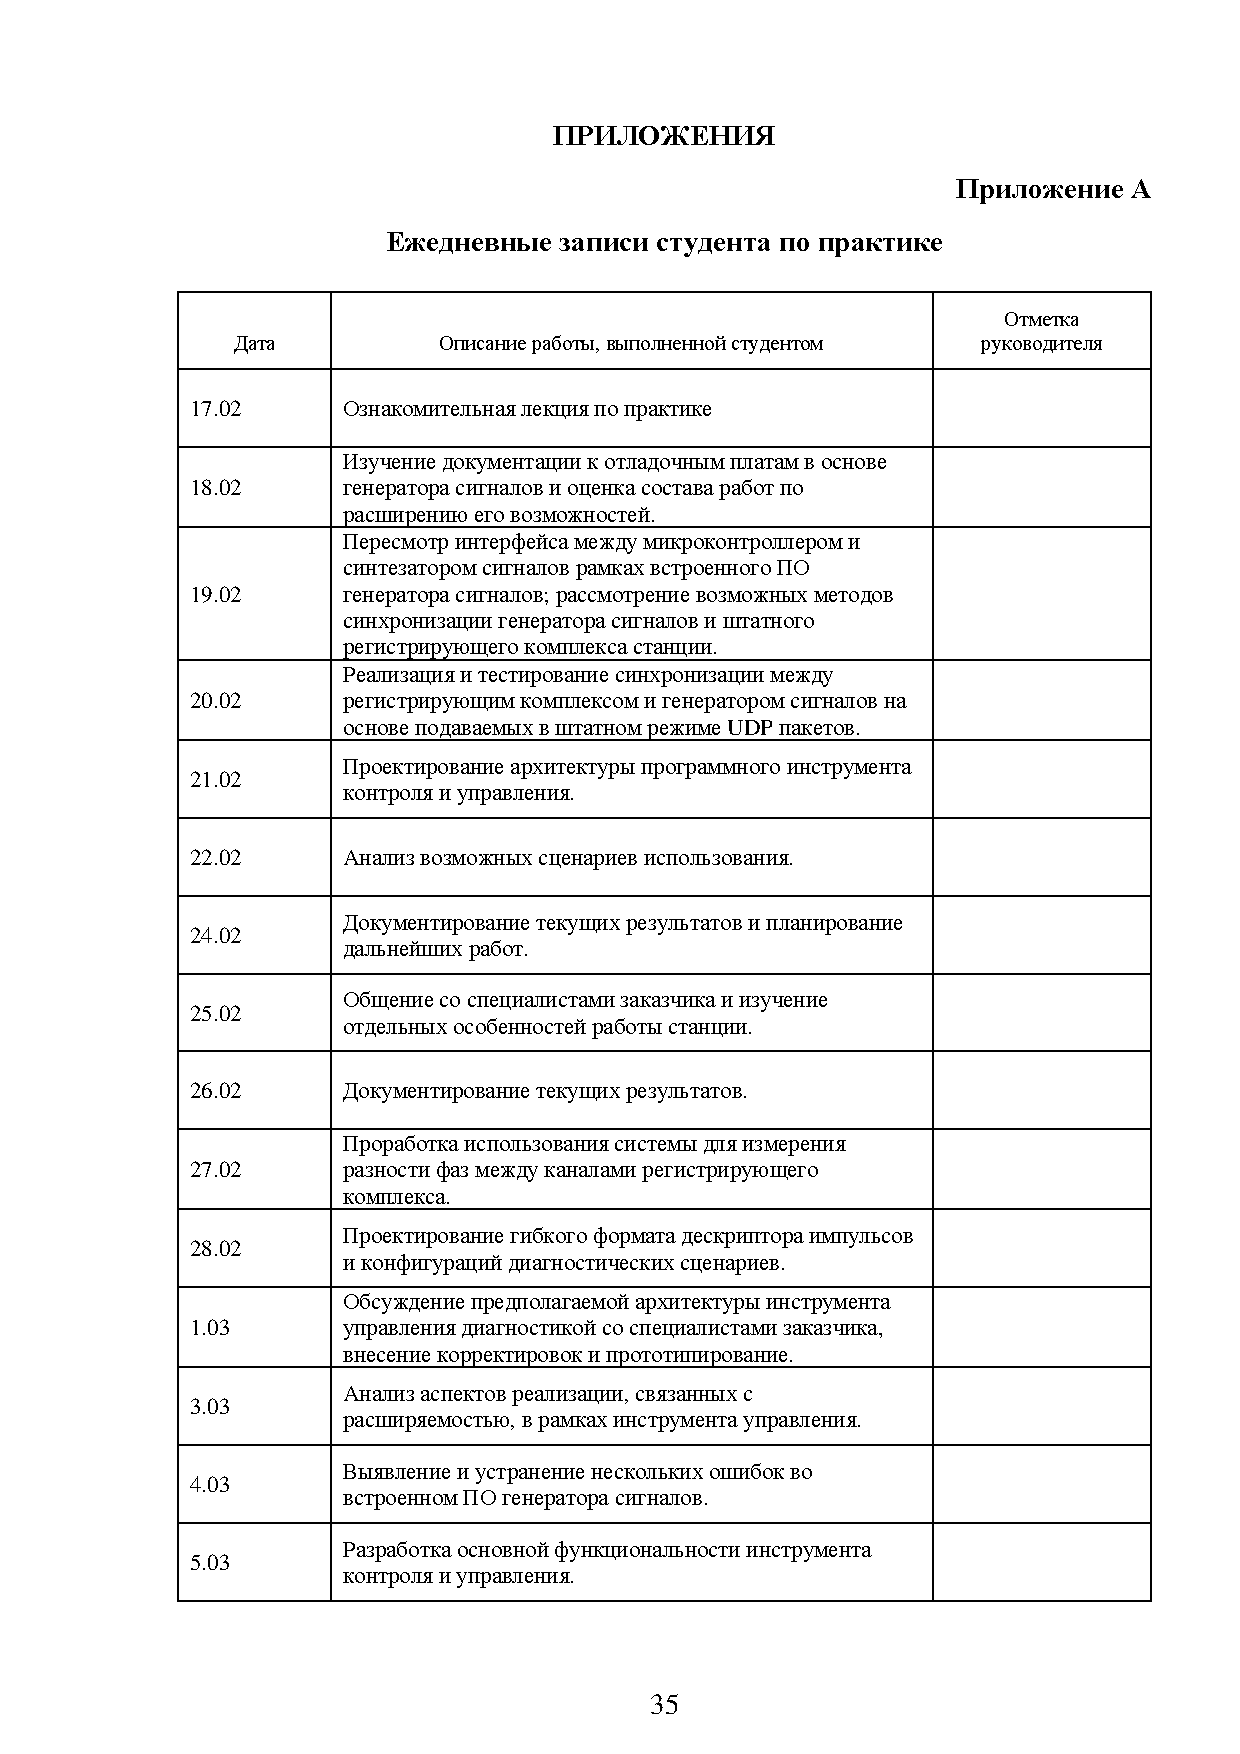
\includepdf[pages={-}, addtotoc={1, chapter, 1, ПРИЛОЖЕНИЯ, extras, 1, section, 1, Приложение А Ежедневные записи студента по практике, asd}]{zapisi.pdf} % файл конвертированный из docx с таблицей и всеми заголовками + номер страницы(!)

\end{document}

